\documentclass[10pt,fleqn]{article}
\usepackage{hyperref}
\usepackage{graphicx}


\setlength{\topmargin}{-.75in}
\addtolength{\textheight}{2.00in}
\setlength{\oddsidemargin}{.00in}
\addtolength{\textwidth}{.75in}

\nofiles

\pagestyle{empty}

\setlength{\parindent}{0in}

% new math commands


\setlength{\oddsidemargin}{-0.25in}
\setlength{\evensidemargin}{-0.25in}
\setlength{\textwidth}{6.75in}
\setlength{\headheight}{0.0in}
\setlength{\topmargin}{-0.25in}
\setlength{\textheight}{9.00in}

\makeindex

\usepackage{mathrsfs}

%\usepackage[pdftex]{graphicx}
\usepackage{epstopdf}

\newcounter{beans}

\newcommand{\ds}{\displaystyle}
\newcommand{\limit}[2]{\displaystyle\lim_{#1\to#2}}

\newcommand{\binomial}[2]{\ \left( \begin{array}{c}
                                  #1 \\
                                  #2
                                 \end{array}
                            \right) \
                         }
\newcommand{\ExampleRule}[2]
  {
  \noindent
  \rule{\linewidth}{1pt}
  \begin{example}
    #1
    \label{#2}
  \end{example}
  \rule{\linewidth}{1pt}
  \vskip0.125in
  }

\newcommand{\defbox}[1]
  {
   \ \\
   \noindent
   \setlength\fboxrule{1pt}
   \fbox{
        \begin{minipage}{6.5in}
          #1
        \end{minipage}
        }
   \ \\
  }
\newcommand{\verysmallworkbox}[1]
  {
   \ \\
   \noindent
   \setlength\fboxrule{1pt}
   \fbox{
        \begin{minipage}{6.5in}
           #1
           \ \\
           \vskip0.5in \ \\
           \ \\
        \end{minipage}
        }
   \ \\
  }
\newcommand{\smallworkbox}[1]
  {
   \ \\
   \noindent
   \setlength\fboxrule{1pt}
   \fbox{
        \begin{minipage}{6.5in}
           #1
           \ \\
           \vskip2.5in \ \\
           \ \\
        \end{minipage}
        }
   \ \\
  }
\newcommand{\halfworkbox}[1]
  {
   \ \\
   \noindent
   \setlength\fboxrule{1pt}
   \fbox{
        \begin{minipage}{6.5in}
           #1 \hfill
           \ \\
           \vskip3.25in \ \\
           \ \\
        \end{minipage}
        }
   \ \\
  }
\newcommand{\largeworkbox}[1]
  {
   \ \\
   \noindent
   \setlength\fboxrule{1pt}
   \fbox{
        \begin{minipage}{6.5in}
           #1
           \ \\
           \vskip7.5in \ \\
           \ \\
        \end{minipage}
        }
   \ \\
  }
\newcommand{\flexworkbox}[2]
  {
   \ \\
   \noindent
   \setlength\fboxrule{1pt}
   \fbox{
        \begin{minipage}{6.5in}
           #1
           \ \\

           \vskip#2 \ \\
           \ \\
        \end{minipage}
        }
   \ \\
  }


% symbols for sets of numbers

\newcommand{\natnumb}{$\cal N$}
\newcommand{\whonumb}{$\cal W$}
\newcommand{\intnumb}{$\cal Z$}
\newcommand{\ratnumb}{$\cal Q$}
\newcommand{\irrnumb}{$\cal I$}
\newcommand{\realnumb}{$\cal R$}
\newcommand{\cmplxnumb}{$\cal C$}

% misc. commands

\newcommand{\mma}{{\it Mathematica}}
\newcommand{\sech}{\mbox{ sech}}
 
\newtheorem{theorem}{Theorem}
\newtheorem{example}{Example}
\newtheorem{definition}{Definition}
\newtheorem{problem}{Problem}

\setcounter{secnumdepth}{2}
\setcounter{tocdepth}{4}


\begin{document}
%%%%%%%%%%%%%%%%%%%%%%%%%%%%%%%%%%%%%%%%%%%%%%%%%%%%%%%%%%%%%%%%%%%%%%%%%%%%%%%%
%%%%%%%%%%%%%%%%%%%%%%%%%%%%%%%%%%%%%%%%%%%%%%%%%%%%%%%%%%%%%%%%%%%%%%%%%%%%%%%%
\vskip0.1in\hrule\vskip0.1in
\noindent
{\bf Math 4610 Fundamentals of Computational Mathematics  - Topic 4.}
\vskip0.1in\hrule\vskip0.1in

This topic covers information on how to work once a terminal is up and running
on your computer. A Linux/Unix operating system should be running in the
terminal. In most real computational settings, it is important to be able to
work using a command line to create files, modify these files, compile
code, and a number of other tasks. You can invoke multiple terminals and work on
multiple files at the same time. Your instructor has three or four terminals
open at any given time. One to edit files, one to compile and execute code, and
the third to display results. The homework and projects assigned in the class
will typically require the use of a terminal to complete the work.

We will eventually use High Performance Computing (HPC) resources at the Center
for High Performance Computing (CHPC) at the University of Utah to work on a
project or two. The access we will have will be through the terminals or
terminal emulators running Linux/Unix operating systems. So, it is important to
be familiar with at least a few basic Linux/Unix commands. In this section of
the notes we will work through a few of the more important commands needed. We
will also introduce more commands with options as we work through the semester.





This topic will cover the various ways to get a
terminal up and running. Once we have a few choices, the notes will focus on
terminals generated by Cygwin and Xtra-PC. Cygwin is freely available for use
on PCs. The instructions on the installation of Cygwin can be found at
\begin{verbatim}

    https://cygwin.org

\end{verbatim}
There are simple instructions to get the installation underway. Note that the
installation of Cygwin on your computer is both a time intensive job and also
requires a bit of disk space. The Xtra-PC platform is stored on a thumb drive
that can be plugged into your PC. It costs a little, but works very well.

The benefits of a Cygwin installation are (1) you get a bunch of compilers (gcc,
gfortran, and others) for coding up algorithms we will cover in the course, (2)
\LaTeX can be installed and used directly. There are a ton of packages available
for you to explore and use. We will also use git which is installed as a part of
Cygwin. With the Xtra-PC version you will likely need to install a few things.
This is also very easy to do.

So, let's start into the various ways to start up a terminal and a couple of
basic commands to execute in the terminal.

\vskip0.1in\hrule\vskip0.1in
{\bf A Brief Introduction to Linux/Unix Emulation with Cygwin:}
\vskip0.1in\hrule\vskip0.1in
\noindent
If you are interested in using Cygwin to pull up a terminal the first thing to
do is to install the software locally. Note that the Engineering Computer Lab
already has a version of Cygwin installed for student use. In a browser, the
first thing you will see is the following.
\vskip0.1in\hrule\vskip0.1in
\vfill
\begin{figure}[h]
\centering
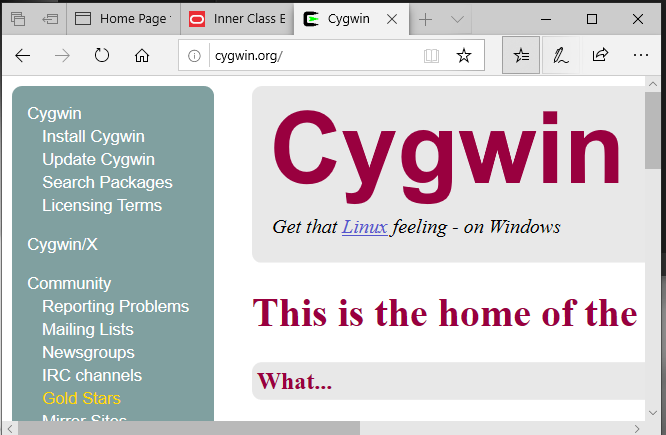
\includegraphics[width=6.0in]{../images/cygwin_00.png}
\vskip0.1in
\caption{Website for installation of Cygwin. {Screenshot} taken using
         {\bf Snip \& Sketch}. This is an app on my Windows 10 box}
\end{figure}
\eject
\vskip0.1in\hrule\vskip0.1in
\noindent
You should start with the base installation if you are not used to installing
large software packages on your computer. After the installation, there should
be an icon on your desktop that can be used to bring up a terminal emulator.
\vskip0.1in\hrule\vskip0.1in
\vfill
\begin{figure}[h]
\centering
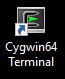
\includegraphics[width=2.0in]{../images/cygwin_icon.png}
\caption{Cygwin icon on your desktop. {Screenshot} taken using
        {\bf Snip \& Sketch}. This is an app on my Windows 10 box}
\end{figure}
\eject
\vskip0.1in\hrule\vskip0.1in
Double click on the icon and a terminal that looks like the following will
appear on your screen. The terminal comes up with a prompt that is based on the
computer name. A basic terminal will start up using the bash command terminal. 
\vskip0.1in\hrule\vskip0.1in
\vfill
\begin{figure}[h]
\centering
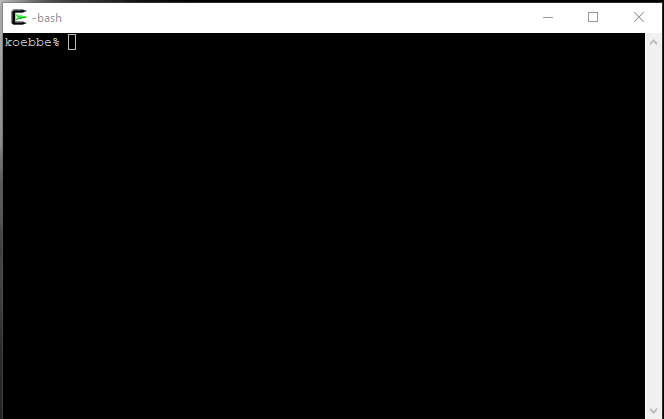
\includegraphics[width=6.0in]{../images/cygwin_01.png}
\caption{Example of a terminal that enulates a Linux operating system and
        command line. {Screenshot} taken using {\bf Snip \& Sketch}. This is
        an app on my Windows 10 box}
\end{figure}
\eject
\vskip0.1in\hrule\vskip0.1in
The text that automatically appears in the terminal is called a prompt. That
is,
\begin{verbatim}

    koebbe%

\end{verbatim}
is the prompt and our job will be to enter commands to get our computer to 
create files, modify files, compile computer programs and the like. The next
topic in our list will give you a few standard commands that can be used to
do real work for the course.
\end{document}





\documentclass[10pt,fleqn]{article}
\usepackage{hyperref}


\setlength{\topmargin}{-.75in}
\addtolength{\textheight}{2.00in}
\setlength{\oddsidemargin}{.00in}
\addtolength{\textwidth}{.75in}

\nofiles

\pagestyle{empty}

\setlength{\parindent}{0in}

% new math commands


\setlength{\oddsidemargin}{-0.25in}
\setlength{\evensidemargin}{-0.25in}
\setlength{\textwidth}{6.75in}
\setlength{\headheight}{0.0in}
\setlength{\topmargin}{-0.25in}
\setlength{\textheight}{9.00in}

\makeindex

\usepackage{mathrsfs}

%\usepackage[pdftex]{graphicx}
\usepackage{epstopdf}

\newcounter{beans}

\newcommand{\ds}{\displaystyle}
\newcommand{\limit}[2]{\displaystyle\lim_{#1\to#2}}

\newcommand{\binomial}[2]{\ \left( \begin{array}{c}
                                  #1 \\
                                  #2
                                 \end{array}
                            \right) \
                         }
\newcommand{\ExampleRule}[2]
  {
  \noindent
  \rule{\linewidth}{1pt}
  \begin{example}
    #1
    \label{#2}
  \end{example}
  \rule{\linewidth}{1pt}
  \vskip0.125in
  }

\newcommand{\defbox}[1]
  {
   \ \\
   \noindent
   \setlength\fboxrule{1pt}
   \fbox{
        \begin{minipage}{6.5in}
          #1
        \end{minipage}
        }
   \ \\
  }
\newcommand{\verysmallworkbox}[1]
  {
   \ \\
   \noindent
   \setlength\fboxrule{1pt}
   \fbox{
        \begin{minipage}{6.5in}
           #1
           \ \\
           \vskip0.5in \ \\
           \ \\
        \end{minipage}
        }
   \ \\
  }
\newcommand{\smallworkbox}[1]
  {
   \ \\
   \noindent
   \setlength\fboxrule{1pt}
   \fbox{
        \begin{minipage}{6.5in}
           #1
           \ \\
           \vskip2.5in \ \\
           \ \\
        \end{minipage}
        }
   \ \\
  }
\newcommand{\halfworkbox}[1]
  {
   \ \\
   \noindent
   \setlength\fboxrule{1pt}
   \fbox{
        \begin{minipage}{6.5in}
           #1 \hfill
           \ \\
           \vskip3.25in \ \\
           \ \\
        \end{minipage}
        }
   \ \\
  }
\newcommand{\largeworkbox}[1]
  {
   \ \\
   \noindent
   \setlength\fboxrule{1pt}
   \fbox{
        \begin{minipage}{6.5in}
           #1
           \ \\
           \vskip7.5in \ \\
           \ \\
        \end{minipage}
        }
   \ \\
  }
\newcommand{\flexworkbox}[2]
  {
   \ \\
   \noindent
   \setlength\fboxrule{1pt}
   \fbox{
        \begin{minipage}{6.5in}
           #1
           \ \\

           \vskip#2 \ \\
           \ \\
        \end{minipage}
        }
   \ \\
  }


% symbols for sets of numbers

\newcommand{\natnumb}{$\cal N$}
\newcommand{\whonumb}{$\cal W$}
\newcommand{\intnumb}{$\cal Z$}
\newcommand{\ratnumb}{$\cal Q$}
\newcommand{\irrnumb}{$\cal I$}
\newcommand{\realnumb}{$\cal R$}
\newcommand{\cmplxnumb}{$\cal C$}

% misc. commands

\newcommand{\mma}{{\it Mathematica}}
\newcommand{\sech}{\mbox{ sech}}
 
\newtheorem{theorem}{Theorem}
\newtheorem{example}{Example}
\newtheorem{definition}{Definition}
\newtheorem{problem}{Problem}

\setcounter{secnumdepth}{2}
\setcounter{tocdepth}{4}


\begin{document}
%%%%%%%%%%%%%%%%%%%%%%%%%%%%%%%%%%%%%%%%%%%%%%%%%%%%%%%%%%%%%%%%%%%%%%%%%%%%%%%%
%%%%%%%%%%%%%%%%%%%%%%%%%%%%%%%%%%%%%%%%%%%%%%%%%%%%%%%%%%%%%%%%%%%%%%%%%%%%%%%%
\vskip0.1in\hrule\vskip0.1in
\noindent
{\bf Math 4610 Fundamentals of Computational Mathematics  - Lecture 1.} 
\vskip0.1in\hrule\vskip0.1in
\noindent
The content for each lecture in Math 4610 will be presented in a lecture format
that will follow an outline presented at the beginning of each class period.
For the first lecture, the following list of items will be covered:
%%%%%%%%%%%%%%%%%%%%%%%%%%%%%%%%%%%%%%%%%%%%%%%%%%%%%%%%%%%%%%%%%%%%%%%%%%%%%%%%
%%%%%%%%%%%%%%%%%%%%%%%%%%%%%%%%%%%%%%%%%%%%%%%%%%%%%%%%%%%%%%%%%%%%%%%%%%%%%%%%
\vskip0.1in\hrule\vskip0.1in
\noindent
{\bf Content Items:}
\begin{list}{$\bullet$}{\usecounter{beans} \parsep=0pt \listparindent=0pt
\topsep=0pt \rightmargin=.35in \leftmargin=.35in \labelsep=5 pt
\itemsep=2pt}
  \item {\bf A Brief Introduction to Command Windows and Linux/Unix:} To be
        effective in Math 4610 you will need to be able to work in some command
        window environment. Many of the software applications we will use will
        require Linux/Unix emulation at a minimum. You are encouraged to install
        Cygwin on your computer if you have enough space. If you are running
        on a Linux machine there is no need to download and install Cygwin.
        Also, if you are using a Mac, the desktop system is already built on a
        Unix kernel. So, there are ready made ways to interact with Unix on a
        Mac/Appled. One such example is Homebrew.
        \href{https://jvkoebbe.github.io/math4610/lectures/lecture_01/md/cygwin_primer}{$>$ $>$ go there}
        \href{https://jvkoebbe.github.io/math4610/lectures/lecture_01/pdf/cygwin_primer.pdf}{(pdf)}
  \item {\bf Compiling and Running a Simple Code - Hello World:} As a simple
        example, how to compile and run a simple code in the C programming
        language will be presented. This will be related to the command window
        primer in the lecture.
        \href{https://jvkoebbe.github.io/math4610/lectures/lecture_01/md/coding_example}{$>$ $>$ go there}
        \href{https://jvkoebbe.github.io/math4610/lectures/lecture_01/pdf/coding_example}{(pdf)}
  \item {\bf Github and Homework:} You will need to create a student account on
        Github for this course. You will be required to build and maintain a
        software manual for the computer codes you will write. A specific format
        for your homework repository and the software manual will be discussed.
        \href{https://jvkoebbe.github.io/math4610/lectures/lecture_01/md/github_primer}{$>$ $>$ go there}
        \href{https://jvkoebbe.github.io/math4610/lectures/lecture_01/pdf/github_primer.pdf}{(pdf)}
  \item {\bf Homework Tasksheets:} Homework for the course will be given via
        tasksheets for students to complete. These task sheets will appear on
        Github for this course. The table of contents for the tasksheets can be
        found through the following links.
        \href{https://jvkoebbe.github.io/math4610/tasksheets/md/toc_tasksheets}{$>$ $>$ go there}
        \href{https://jvkoebbe.github.io/math4610/tasksheets/pdf/toc_tasksheet.pdf}{(pdf)}
  \item {\bf Wrap up and Questions:} If there is time and anyone has questions
        about the lecture, these will be addressed.
\end{list}
\vskip0.1in\hrule\vskip0.1in
%%%%%%%%%%%%%%%%%%%%%%%%%%%%%%%%%%%%%%%%%%%%%%%%%%%%%%%%%%%%%%%%%%%%%%%%%%%%%%%%
%%%%%%%%%%%%%%%%%%%%%%%%%%%%%%%%%%%%%%%%%%%%%%%%%%%%%%%%%%%%%%%%%%%%%%%%%%%%%%%%
\end{document}
\documentclass[10pt,fleqn]{article}
%\usepackage{graphicx}


\setlength{\topmargin}{-.75in}
\addtolength{\textheight}{2.00in}
\setlength{\oddsidemargin}{.00in}
\addtolength{\textwidth}{.75in}

\nofiles

\pagestyle{empty}

\setlength{\parindent}{0in}

% new math commands


\setlength{\oddsidemargin}{-0.25in}
\setlength{\evensidemargin}{-0.25in}
\setlength{\textwidth}{6.75in}
\setlength{\headheight}{0.0in}
\setlength{\topmargin}{-0.25in}
\setlength{\textheight}{9.00in}

\makeindex

\usepackage{mathrsfs}

%\usepackage[pdftex]{graphicx}
\usepackage{epstopdf}

\newcounter{beans}

\newcommand{\ds}{\displaystyle}
\newcommand{\limit}[2]{\displaystyle\lim_{#1\to#2}}

\newcommand{\binomial}[2]{\ \left( \begin{array}{c}
                                  #1 \\
                                  #2
                                 \end{array}
                            \right) \
                         }
\newcommand{\ExampleRule}[2]
  {
  \noindent
  \rule{\linewidth}{1pt}
  \begin{example}
    #1
    \label{#2}
  \end{example}
  \rule{\linewidth}{1pt}
  \vskip0.125in
  }

\newcommand{\defbox}[1]
  {
   \ \\
   \noindent
   \setlength\fboxrule{1pt}
   \fbox{
        \begin{minipage}{6.5in}
          #1
        \end{minipage}
        }
   \ \\
  }
\newcommand{\verysmallworkbox}[1]
  {
   \ \\
   \noindent
   \setlength\fboxrule{1pt}
   \fbox{
        \begin{minipage}{6.5in}
           #1
           \ \\
           \vskip0.5in \ \\
           \ \\
        \end{minipage}
        }
   \ \\
  }
\newcommand{\smallworkbox}[1]
  {
   \ \\
   \noindent
   \setlength\fboxrule{1pt}
   \fbox{
        \begin{minipage}{6.5in}
           #1
           \ \\
           \vskip2.5in \ \\
           \ \\
        \end{minipage}
        }
   \ \\
  }
\newcommand{\halfworkbox}[1]
  {
   \ \\
   \noindent
   \setlength\fboxrule{1pt}
   \fbox{
        \begin{minipage}{6.5in}
           #1 \hfill
           \ \\
           \vskip3.25in \ \\
           \ \\
        \end{minipage}
        }
   \ \\
  }
\newcommand{\largeworkbox}[1]
  {
   \ \\
   \noindent
   \setlength\fboxrule{1pt}
   \fbox{
        \begin{minipage}{6.5in}
           #1
           \ \\
           \vskip7.5in \ \\
           \ \\
        \end{minipage}
        }
   \ \\
  }
\newcommand{\flexworkbox}[2]
  {
   \ \\
   \noindent
   \setlength\fboxrule{1pt}
   \fbox{
        \begin{minipage}{6.5in}
           #1
           \ \\

           \vskip#2 \ \\
           \ \\
        \end{minipage}
        }
   \ \\
  }


% symbols for sets of numbers

\newcommand{\natnumb}{$\cal N$}
\newcommand{\whonumb}{$\cal W$}
\newcommand{\intnumb}{$\cal Z$}
\newcommand{\ratnumb}{$\cal Q$}
\newcommand{\irrnumb}{$\cal I$}
\newcommand{\realnumb}{$\cal R$}
\newcommand{\cmplxnumb}{$\cal C$}

% misc. commands

\newcommand{\mma}{{\it Mathematica}}
\newcommand{\sech}{\mbox{ sech}}
 
\newtheorem{theorem}{Theorem}
\newtheorem{example}{Example}
\newtheorem{definition}{Definition}
\newtheorem{problem}{Problem}

\setcounter{secnumdepth}{2}
\setcounter{tocdepth}{4}


\begin{document}
%%%%%%%%%%%%%%%%%%%%%%%%%%%%%%%%%%%%%%%%%%%%%%%%%%%%%%%%%%%%%%%%%%%%%%%%%%%%%%%%
%%%%%%%%%%%%%%%%%%%%%%%%%%%%%%%%%%%%%%%%%%%%%%%%%%%%%%%%%%%%%%%%%%%%%%%%%%%%%%%%
\vskip0.1in\hrule\vskip0.1in
\noindent
{\bf Math 4610 Fundamentals of Computational Mathematics  - Lecture 1.} 
\vskip0.1in\hrule\vskip0.1in
\noindent
The content for each lecture in Math 4610 will be presented in a lecture format
that will follow an outline presented at the beginning of each class period.
For the first lecture, the following list of items will be covered:
%%%%%%%%%%%%%%%%%%%%%%%%%%%%%%%%%%%%%%%%%%%%%%%%%%%%%%%%%%%%%%%%%%%%%%%%%%%%%%%%
%%%%%%%%%%%%%%%%%%%%%%%%%%%%%%%%%%%%%%%%%%%%%%%%%%%%%%%%%%%%%%%%%%%%%%%%%%%%%%%%
\vskip0.1in\hrule\vskip0.1in
\noindent
{\bf Content Items:}
\begin{list}{$\bullet$}{\usecounter{beans} \parsep=0pt \listparindent=0pt
\topsep=0pt \rightmargin=.35in \leftmargin=.35in \labelsep=5 pt
\itemsep=2pt}
  \item {\bf The Syllabus:} As in any college course, the syllabus in this
        course will provide students with an idea of what is expected. The
        syllabus in this course will cover instructor information, instructor
        comments and policies, grading information, and some information about
        university poliocies.
  \item {\bf Using Version Control Systems (VCS) - git:} A brief discussion of
        \lq git\rq\ will be discussed in class to show how to work and
        collaborate with other students and your instructor.
  \item {\bf Github and Homework:} You will need to create a student account on
        Github for this course. You will be required to build and maintain a
        software manual for the computer codes you will write. A specific format
        for your homework repository and the software manual will be discussed.
  \item {\bf Wrap up and Questions:} If there is time and anyone has questions
        about the lecture, these will be addressed.
\end{list}
\vskip0.1in\hrule\vskip0.1in
%%%%%%%%%%%%%%%%%%%%%%%%%%%%%%%%%%%%%%%%%%%%%%%%%%%%%%%%%%%%%%%%%%%%%%%%%%%%%%%%
%%%%%%%%%%%%%%%%%%%%%%%%%%%%%%%%%%%%%%%%%%%%%%%%%%%%%%%%%%%%%%%%%%%%%%%%%%%%%%%%
\end{document}
\documentclass[10pt,fleqn]{article}
%\usepackage{graphicx}


\setlength{\topmargin}{-.75in}
\addtolength{\textheight}{2.00in}
\setlength{\oddsidemargin}{.00in}
\addtolength{\textwidth}{.75in}

\title{Math 4610 Lecture Notes \\
            \ \\
       A Brief Introduction to Cygwin Usage
  \footnote{These notes are part of an Open Resource Educational project
            sponsored by Utah State University}}

\author{Joe Koebbe}

\nofiles

\pagestyle{empty}

\setlength{\parindent}{0in}

% new math commands


\setlength{\oddsidemargin}{-0.25in}
\setlength{\evensidemargin}{-0.25in}
\setlength{\textwidth}{6.75in}
\setlength{\headheight}{0.0in}
\setlength{\topmargin}{-0.25in}
\setlength{\textheight}{9.00in}

\makeindex

\usepackage{mathrsfs}

%\usepackage[pdftex]{graphicx}
\usepackage{epstopdf}

\newcounter{beans}

\newcommand{\ds}{\displaystyle}
\newcommand{\limit}[2]{\displaystyle\lim_{#1\to#2}}

\newcommand{\binomial}[2]{\ \left( \begin{array}{c}
                                  #1 \\
                                  #2
                                 \end{array}
                            \right) \
                         }
\newcommand{\ExampleRule}[2]
  {
  \noindent
  \rule{\linewidth}{1pt}
  \begin{example}
    #1
    \label{#2}
  \end{example}
  \rule{\linewidth}{1pt}
  \vskip0.125in
  }

\newcommand{\defbox}[1]
  {
   \ \\
   \noindent
   \setlength\fboxrule{1pt}
   \fbox{
        \begin{minipage}{6.5in}
          #1
        \end{minipage}
        }
   \ \\
  }
\newcommand{\verysmallworkbox}[1]
  {
   \ \\
   \noindent
   \setlength\fboxrule{1pt}
   \fbox{
        \begin{minipage}{6.5in}
           #1
           \ \\
           \vskip0.5in \ \\
           \ \\
        \end{minipage}
        }
   \ \\
  }
\newcommand{\smallworkbox}[1]
  {
   \ \\
   \noindent
   \setlength\fboxrule{1pt}
   \fbox{
        \begin{minipage}{6.5in}
           #1
           \ \\
           \vskip2.5in \ \\
           \ \\
        \end{minipage}
        }
   \ \\
  }
\newcommand{\halfworkbox}[1]
  {
   \ \\
   \noindent
   \setlength\fboxrule{1pt}
   \fbox{
        \begin{minipage}{6.5in}
           #1 \hfill
           \ \\
           \vskip3.25in \ \\
           \ \\
        \end{minipage}
        }
   \ \\
  }
\newcommand{\largeworkbox}[1]
  {
   \ \\
   \noindent
   \setlength\fboxrule{1pt}
   \fbox{
        \begin{minipage}{6.5in}
           #1
           \ \\
           \vskip7.5in \ \\
           \ \\
        \end{minipage}
        }
   \ \\
  }
\newcommand{\flexworkbox}[2]
  {
   \ \\
   \noindent
   \setlength\fboxrule{1pt}
   \fbox{
        \begin{minipage}{6.5in}
           #1
           \ \\

           \vskip#2 \ \\
           \ \\
        \end{minipage}
        }
   \ \\
  }


% symbols for sets of numbers

\newcommand{\natnumb}{$\cal N$}
\newcommand{\whonumb}{$\cal W$}
\newcommand{\intnumb}{$\cal Z$}
\newcommand{\ratnumb}{$\cal Q$}
\newcommand{\irrnumb}{$\cal I$}
\newcommand{\realnumb}{$\cal R$}
\newcommand{\cmplxnumb}{$\cal C$}

% misc. commands

\newcommand{\mma}{{\it Mathematica}}
\newcommand{\sech}{\mbox{ sech}}
 
\newtheorem{theorem}{Theorem}
\newtheorem{example}{Example}
\newtheorem{definition}{Definition}
\newtheorem{problem}{Problem}

\setcounter{secnumdepth}{2}
\setcounter{tocdepth}{4}


\begin{document}
\maketitle
\newpage
%%%%%%%%%%%%%%%%%%%%%%%%%%%%%%%%%%%%%%%%%%%%%%%%%%%%%%%%%%%%%%%%%%%%%%%%%%%%%%%%
%%%%%%%%%%%%%%%%%%%%%%%%%%%%%%%%%%%%%%%%%%%%%%%%%%%%%%%%%%%%%%%%%%%%%%%%%%%%%%%%

%%%%%%%%%%%%%%%%%%%%%%%%%%%%%%%%%%%%%%%%%%%%%%%%%%%%%%%%%%%%%%%%%%%%%%%%%%%%%%%%
%%%%%%%%%%%%%%%%%%%%%%%%%%%%%%%%%%%%%%%%%%%%%%%%%%%%%%%%%%%%%%%%%%%%%%%%%%%%%%%%
\vskip0.1in\hrule\vskip0.1in
\noindent
{\bf Cygwin Primer for Math 4610 at USU: Just Some Basic Commands} 
\vskip0.1in\hrule\vskip0.1in
\noindent
To install Cygwin on your computer, first find the web site:
\begin{verbatim}

   cygwin.org

\end{verbatim}
The following shows what will pop up when you use a browser to get to the site.
There are instructions for downloading and installing the packages you will need
for the course. Your instructor downloads and saves the setup-x86\_64.exe file
for an installation on a laptop or desktop. Double click on the file once you
have saved the file. Note that the installation will take a bit of time and
diskspace. There is an image below that shows what the desktop icon looks like.
%%%%%%%%%%%%%%%%%%%%%%%%%%%%%%%%%%%%%%%%%%%%%%%%%%%%%%%%%%%%%%%%%%%%%%%%%%%%%%%%
%%%%%%%%%%%%%%%%%%%%%%%%%%%%%%%%%%%%%%%%%%%%%%%%%%%%%%%%%%%%%%%%%%%%%%%%%%%%%%%%
\vskip0.1in\hrule\vskip0.1in
\noindent
{{\bf Cygwin Primer for Math 4610 at USU:} Getting a Cygwin Terminal Up and
   Running} 
\vskip0.1in\hrule\vskip0.1in
\noindent
Cygwin can be installed on just about any computer. If you are working on a
Linux or Unix system you won't need to install Cygwin. Cygwin can be a huge
storage hog if you install everything in the package. You can install a basic
version that takes up less disk space. Also, the computer lab on the third
floor of the Engineering  Building has Cygwin installed and running if this
option is needed. Once you have a version of Cygwin available, you can double
click the icon on the Desktop or in the list apps on a Windows machine to
obtain a terminal to work in, see below.
%%%%%%%%%%%%%%%%%%%%%%%%%%%%%%%%%%%%%%%%%%%%%%%%%%%%%%%%%%%%%%%%%%%%%%%%%%%%%%%%
%%%%%%%%%%%%%%%%%%%%%%%%%%%%%%%%%%%%%%%%%%%%%%%%%%%%%%%%%%%%%%%%%%%%%%%%%%%%%%%%
\vskip0.1in\hrule\vskip0.1in
\noindent
{{\bf Cygwin Primer for Math 4610 at USU:} List the Contents of the Home
    Directory} 
\vskip0.1in\hrule\vskip0.1in
\noindent
The first thing to look at is what is in a directory. It is important to know
where you are at in a directory and the like. This also serves as a first linux
or unix command. In the screenshot below there are a couple of versions of a
command that will list files and folders with more or less information. Note
that most linux commands look like the following:
\begin{verbatim}

   % command [options] [input parameters]

\end{verbatim}
\vskip0.1in\hrule\vskip0.1in
\vfill
\begin{figure}[h]
\centering
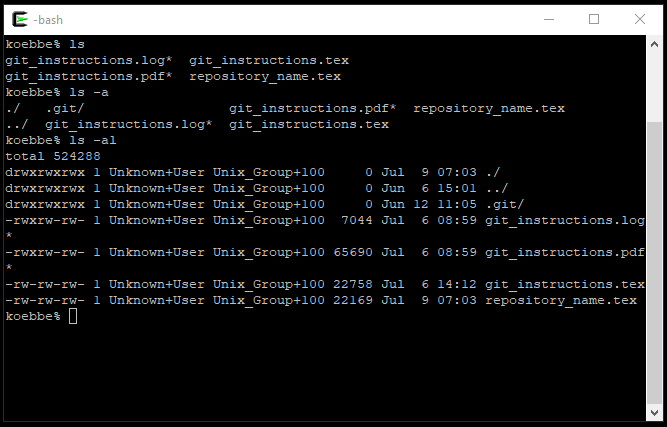
\includegraphics{../images/cygwin_02.png}
\caption{{Screenshot} taken using {\bf Snip \& Sketch}. This is an app on
         my Windows 10 box}
\end{figure}
\eject
%%%%%%%%%%%%%%%%%%%%%%%%%%%%%%%%%%%%%%%%%%%%%%%%%%%%%%%%%%%%%%%%%%%%%%%%%%%%%%%%
%%%%%%%%%%%%%%%%%%%%%%%%%%%%%%%%%%%%%%%%%%%%%%%%%%%%%%%%%%%%%%%%%%%%%%%%%%%%%%%%
\vskip0.1in\hrule\vskip0.1in
\noindent
{{\bf Cygwin Primer for Math 4610 at USU:} Directory Commands} 
\vskip0.1in\hrule\vskip0.1in
\noindent
You will need to create, move, remove, and other things to directories to keep
work organized. The {\bf mkdir} command allows a persion to create a new
directory in the current working directory. This is the same thing tha Windows
Explorer allows you to do with a popup menu. There will be many places where
a directory structure will be required. You can remove a directory with the
{\bf rmdir} command. The {\bf cd} command can be used to navigate through a
directory structure. Finally, on this screen capture, the {\bf pwd} command is
used to determine the current working directory. This can be used to figure out
where you are in a directory structure.
\begin{verbatim}

    % pwd                 current working directory
    % cd                  change working directory
    % mkdir               make a new directory
    % rmdir               remove an existing directory

\end{verbatim}
\vskip0.1in\hrule\vskip0.1in
\vfill
\begin{figure}[h]
\centering
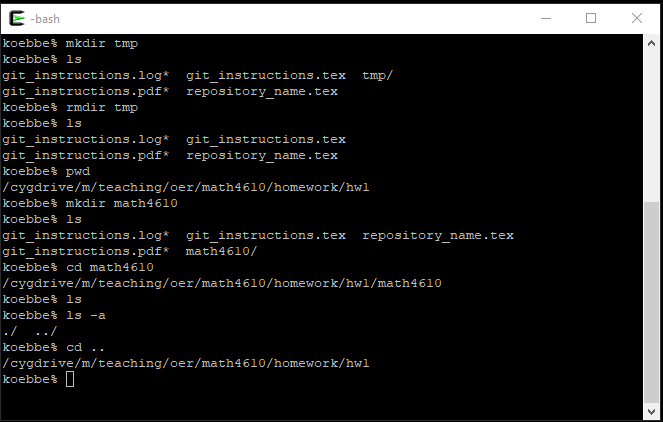
\includegraphics{../images/cygwin_03.png}
\caption{{Screenshot} taken using {\bf Snip \& Sketch}. This is an app on
         my Windows 10 box}
\end{figure}
\eject
%%%%%%%%%%%%%%%%%%%%%%%%%%%%%%%%%%%%%%%%%%%%%%%%%%%%%%%%%%%%%%%%%%%%%%%%%%%%%%%%
%%%%%%%%%%%%%%%%%%%%%%%%%%%%%%%%%%%%%%%%%%%%%%%%%%%%%%%%%%%%%%%%%%%%%%%%%%%%%%%%
\vskip0.1in\hrule\vskip0.1in
\noindent
{{\bf Cygwin Primer for Math 4610 at USU:} Which Command} 
\vskip0.1in\hrule\vskip0.1in
\noindent
You will want to know what is available for doing work within Cygwin or any
other platform. The which command will let you know if apps or other executables
are available on your version of Cygwin. In particular, it is important to know
if certain compilers (e.g, javac, gcc, f77) are available. A significant number
of tasks you will be asked to complete will require the use of a compiler and
Cygwin has a number of (good) standard compilers for C, C++, and fortran. The
syntax for the command is the following.
\begin{verbatim}

    % which command

\end{verbatim}
\vskip0.1in\hrule\vskip0.1in
\vfill
\begin{figure}[h]
\centering
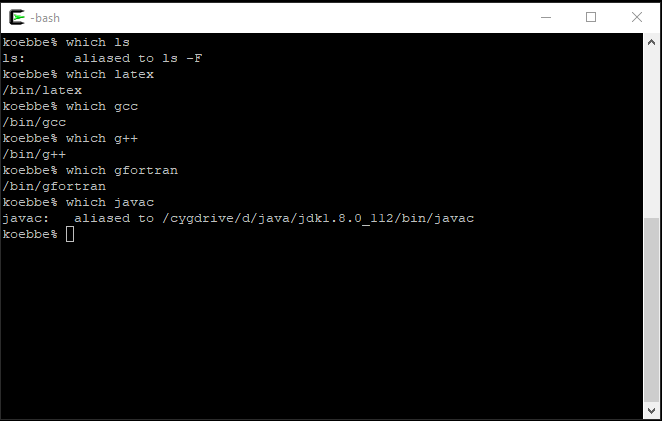
\includegraphics{../images/cygwin_04.png}
\caption{{Screenshot} taken using {\bf Snip \& Sketch}. This is an app on
         my Windows 10 box}
\end{figure}
\eject
%%%%%%%%%%%%%%%%%%%%%%%%%%%%%%%%%%%%%%%%%%%%%%%%%%%%%%%%%%%%%%%%%%%%%%%%%%%%%%%%
%%%%%%%%%%%%%%%%%%%%%%%%%%%%%%%%%%%%%%%%%%%%%%%%%%%%%%%%%%%%%%%%%%%%%%%%%%%%%%%%
\vskip0.1in\hrule\vskip0.1in
\noindent
{{\bf Cygwin Primer for Math 4610 at USU:} A Simple Editing Program} 
\vskip0.1in\hrule\vskip0.1in
\noindent
You will need an editor to create text files. There are a number of editors that
can be downloaded and used in any Cygwin installation. The standard editor that
is always available for linux and unix boxes is \lq vi\rq\. This editor is a bit
rudimentary, but works. Another editor which will be used in by the instructor
in the course is \lq vim\rq. The syntax for starting the editor in a window is
the following.
\begin{verbatim}

    % vim filename

\end{verbatim}
There are a lot of escape sequences it insert text, write a file and so on. If
you are new to vim, you will need to learn at least a few of these editing
commands.
\vskip0.1in\hrule\vskip0.1in
\vfill
\begin{figure}[h]
\centering
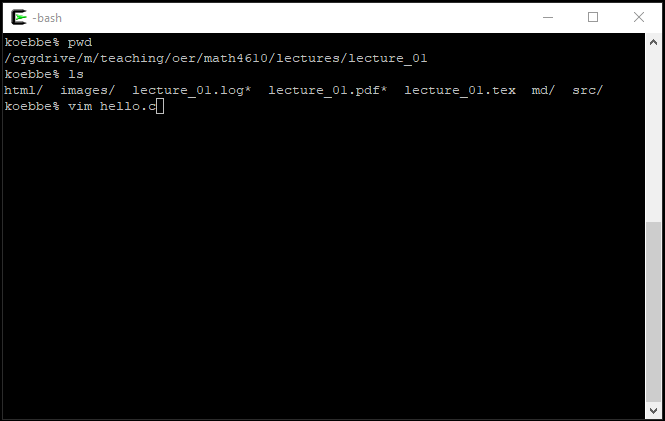
\includegraphics{../images/cygwin_05.png}
\caption{{Screenshot} taken using {\bf Snip \& Sketch}. This is an app on
         my Windows 10 box}
\end{figure}
\eject
%%%%%%%%%%%%%%%%%%%%%%%%%%%%%%%%%%%%%%%%%%%%%%%%%%%%%%%%%%%%%%%%%%%%%%%%%%%%%%%%
%%%%%%%%%%%%%%%%%%%%%%%%%%%%%%%%%%%%%%%%%%%%%%%%%%%%%%%%%%%%%%%%%%%%%%%%%%%%%%%%
\vskip0.1in\hrule\vskip0.1in
\noindent
{{\bf Cygwin Primer for Math 4610 at USU:} First View of the vim Editor} 
\vskip0.1in\hrule\vskip0.1in
\noindent
Below is what the terminal will turn into when you start up the editor on a new
file. To get out of the editor, you can use any of the following commands inside
the editor.
\begin{verbatim}

    :x                  write and exit the editor - saves changes in the file
    :q                  exit the editor if no changes have been made
    :x!                 force a write and exit the editor - saves the file
    :q!                 force an exit of the editor - no changes are saved

\end{verbatim}
Note that there are a few other commands that can be used to save changes. For
example
\begin{verbatim}

    :w                  write and stay in the editor
    :w!                 force a write and stay in the editor

\end{verbatim}
\vskip0.1in\hrule\vskip0.1in
\vfill
\begin{figure}[h]
\centering
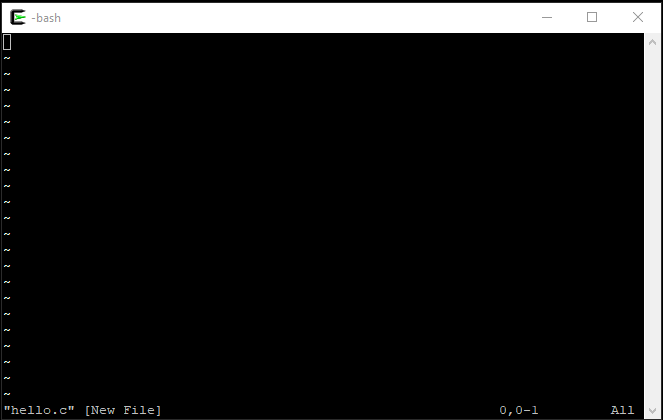
\includegraphics{../images/cygwin_06.png}
\caption{{Screenshot} taken using {\bf Snip \& Sketch}. This is an app on
         my Windows 10 box}
\end{figure}
\eject
%%%%%%%%%%%%%%%%%%%%%%%%%%%%%%%%%%%%%%%%%%%%%%%%%%%%%%%%%%%%%%%%%%%%%%%%%%%%%%%%
%%%%%%%%%%%%%%%%%%%%%%%%%%%%%%%%%%%%%%%%%%%%%%%%%%%%%%%%%%%%%%%%%%%%%%%%%%%%%%%%
\vskip0.1in\hrule\vskip0.1in
\noindent
{{\bf Cygwin Primer for Math 4610 at USU:} An Example of a Text File/Program} 
\vskip0.1in\hrule\vskip0.1in
\noindent
The following screenshot shows a few lines that have been typed into vim that
deinfes a standard hello world example for C. To insert/append characters in the
text file, you can use the following commands to do this. Note that the commands
below do not show up on the screen and the chnages are made where the cursor is
currently located.
\begin{verbatim}

    a                     append text at this point in the file
    o                     open a line after the current line
    O                     open a line before the current line

\end{verbatim}
To end adding or inserting text, use the escape character. Again, the commands
will not show up on screen. Learning everything about vi or vim is a time
consuming process. It is one of those things that you figure out as you go.
\vskip0.1in\hrule\vskip0.1in
\vfill
\begin{figure}[h]
\centering
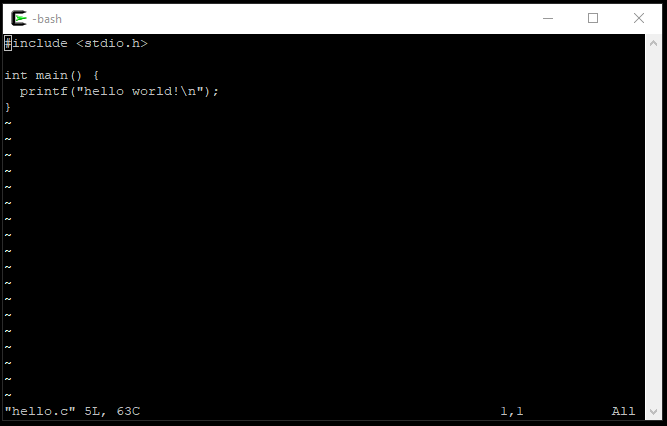
\includegraphics{../images/cygwin_07.png}
\caption{{Screenshot} taken using {\bf Snip \& Sketch}. This is an app on
         my Windows 10 box}
\end{figure}
\eject
%%%%%%%%%%%%%%%%%%%%%%%%%%%%%%%%%%%%%%%%%%%%%%%%%%%%%%%%%%%%%%%%%%%%%%%%%%%%%%%%
%%%%%%%%%%%%%%%%%%%%%%%%%%%%%%%%%%%%%%%%%%%%%%%%%%%%%%%%%%%%%%%%%%%%%%%%%%%%%%%%
\vskip0.1in\hrule\vskip0.1in
\noindent
{{\bf Cygwin Primer for Math 4610 at USU:} Compiling a Program} 
\vskip0.1in\hrule\vskip0.1in
\noindent
Compiling a program is relatively easy at this point in time. To compile the
program on the previous page you should type in
\begin{verbatim}

    % gcc hello.c

\end{verbatim}
The result is an exeutable as seen below. If you want to name the executable
something besides \lq a\rq\ then type the following.
\begin{verbatim}

    % gcc -o hello hello.c

\end{verbatim}
\vskip0.1in\hrule\vskip0.1in
\vfill
\begin{figure}[h]
\centering
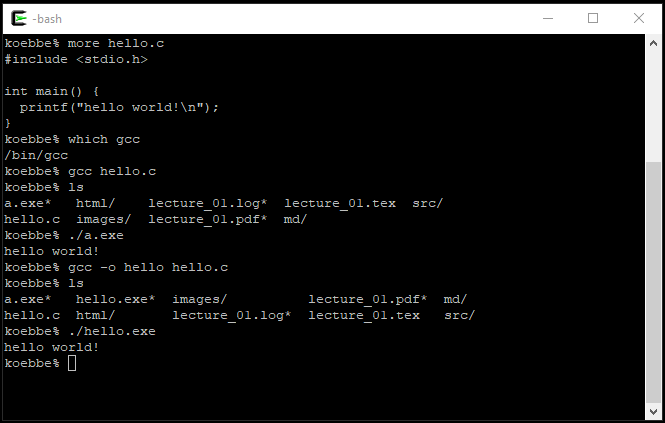
\includegraphics{../images/cygwin_08.png}
\caption{{Screenshot} taken using {\bf Snip \& Sketch}. This is an app on
         my Windows 10 box}
\end{figure}
\eject
%%%%%%%%%%%%%%%%%%%%%%%%%%%%%%%%%%%%%%%%%%%%%%%%%%%%%%%%%%%%%%%%%%%%%%%%%%%%%%%%
%%%%%%%%%%%%%%%%%%%%%%%%%%%%%%%%%%%%%%%%%%%%%%%%%%%%%%%%%%%%%%%%%%%%%%%%%%%%%%%%
\vskip0.1in\hrule\vskip0.1in
\noindent
{{\bf Cygwin Primer for Math 4610 at USU:} Keeping Track of Working Code}
\vskip0.1in\hrule\vskip0.1in
\noindent
It is a good idea to organize your work within assignments and projects. There
is a standard set of folders/directories in linux and unix that most have
adopted. Your instructor follows this idea and usually creates a list of
folders including /src, /data, /bin, and /doc. When computer literate folks see
these folders, they know what is stored in the folders. As an example,
\begin{verbatim}

    % mkdir src
    % mkdir bin

\end{verbatim}
can be used and then the executable the text file can be put into /src and the
binary can be copied into /bin. 
\vskip0.1in\hrule\vskip0.1in
\vfill
\begin{figure}[h]
\centering
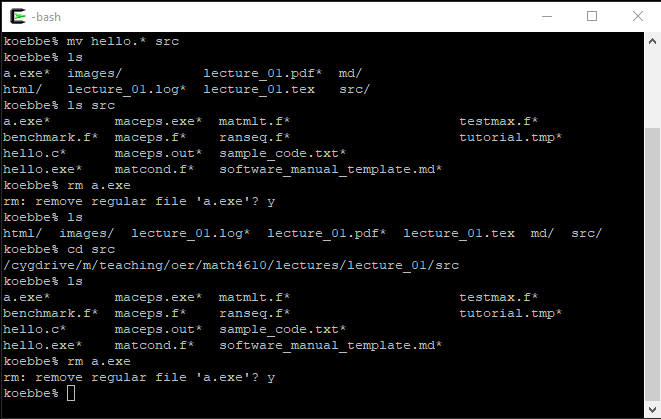
\includegraphics{../images/cygwin_09.png}
\caption{{Screenshot} taken using {\bf Snip \& Sketch}. This is an app on
         my Windows 10 box}
\end{figure}
\eject
%%%%%%%%%%%%%%%%%%%%%%%%%%%%%%%%%%%%%%%%%%%%%%%%%%%%%%%%%%%%%%%%%%%%%%%%%%%%%%%%
%%%%%%%%%%%%%%%%%%%%%%%%%%%%%%%%%%%%%%%%%%%%%%%%%%%%%%%%%%%%%%%%%%%%%%%%%%%%%%%%
\end{document}
